\subsection{Zabbix}

\subsubsection{Motivation}
	The necessity for administrative tasks on great number of computers can be tedious and time consuming without any means of automation or help. As the information on every single computer or system needed to be done one after another separately from each other as the administered systems could vary greatly in both the used hardware and the software which was installed on them. Furthermore with current distributed systems which could span the globe it is further difficult to administer these since there is now also a great distance for the administrator to travel to actually access the systems. Thus arose a need for a program which would support the surveillance and to a certain degree the control of a collection of systems. Such a program should grant the administrator a centralized access to view the status of all necessary systems. These programs were called monitors.
\subsubsection{Monitor}
	The key component of this project is the monitor, which is responsible for the surveillance of the projects systems. A monitors job is the surveillance of certain processes or systems and logging any information or notable occurrences for further analysis. But monitors also have to interfere, control or alert if certain acquired information go beyond estimated or allowed thresholds. Thus the monitors exceed the functionality of simple watchers.\cite{zab1}
\subsubsection{Zabbix}
	Zabbix is such a monitor and thus is tasked with the job of surveying systems for administrative controlling. The surveyed systems can be whole computers, virtual machines within a computing cloud or even network devices. Zabbix is an Open Source monitor licensed under the GPL license and written in programming language\ C\ and thus compiled for a great variety of different operating systems to ensure optimal functionality. It is so to prevent Zabbix from consuming resources which are necessary for other tasks on the surveyed systems, as\ C\ programs compiled for specific systems are specifically tuned for them. For that reason Zabbix splits its functionality into two. The Zabbix server which is tasked with accumulating all the acquired information and data and the Zabbix agent, which other than the Zabbix server is installed directly on the surveyed system, is tasked with gathering information for the server. Zabbix server can receive the input from a great number of agents and thus it is a centralized single monitor service. The Zabbix server stores all the acquired data in its own database, which can be a SQL database, for example MySQL or PostgreSQL. For the ease of access for the gathered data and also for the easier configuration the Zabbix server has a web frontend. The web frontend gives a lot of possibilities to configure and view different data or the surveyed systems and to group and categorize the systems themselves too. But the most important functionality of the Zabbix web frontend is its capability to visualize the stored data values in graphs for easier understandings and readability by its users. From these graphs the user can see the times when the items, so called data representation types within Zabbix, took on which values and thus allow seeing their trending. These items created within the Zabbix server are referenced to a certain system to differentiate the source of the information. To simplify the management these items often can be grouped or combined into templates, which in turn are assigned to systems. Any changes to the items within a template are automatically forwarded to the corresponding items on systems which are referencing these templates. These items can be differentiated into three types, the agent item type, the calculated item type and the trapper item type. The agent item is entirely handled by the Zabbix server and retrieved through the Zabbix agent on the monitored system. The calculated item is also entirely handled by the Zabbix server and is a result of a computed formula which was given to the calculated item from already stored data on the Zabbix server. The trapper item however is an item, which information and values comes from a different source other than the Zabbix agent. Such a trapper items value has to be manually sent to the Zabbix server. Generally Zabbix has two ways to acquire data for its items, by polling or by trapping. Polled data item information is regularly retrieved through a Zabbix server request sent to the Zabbix agent. With trapping Zabbix server is receiving the data irregularly by manual sending from a data source which is using the REST API of Zabbix or the Zabbix own zabbix\_sender command line prompt. The REST API is realized through a JSON remote procedure call while the zabbix\_sender is required to have been installed and can be used in the sending systems terminal. The data values and information sent by the zabbix\_sender and the JSON requests have to be sent manually by the programming environment which is trying to relay information to the Zabbix server. Each time data is received by the Zabbix server it is checked for thresholds in the registered triggers for the specific item, which are responsible for the control, reactions and alerts within Zabbix.\cite{zab2, zab3}
	
	In the context of the project were set requirements for the monitoring which were to be met as to guarantee a minimum level of functionality to work with to accomplish the projects goals. One of the requirements is that the monitoring is to provide an environment for storing, visualizing and managing of essential data. Zabbix solves these through the use of the Zabbix server and its configurable web frontend as centralized access point. Another requirement for monitoring is support for manual data posting and retrieval from its storage. The data retrieval is addressed in Zabbix through its REST API using JSON remote procedure calls while the manual sending could be realized through the same API or using the Zabbix own zabbix\_sender. And the last requirement is that the monitoring be able to react as per definition if data values exceed their thresholds by alerting or interfering. Registered triggers on necessary items are the solution to this requirement in Zabbix. In addition Zabbix is Open Source and thus can be modified if necessary.
\subsubsection{Implementation}
	In the following will be explained the choices made and constructed models in relation to Zabbix in the project.
	After several iterations the data model for the representation of the projects system was split into two separate models. One would model all the data concerning the servers on which our project will be run and the other would model the user specific data. These models were put into corresponding templates for easier modification and assignment of data to newly registered computers in Zabbix.
\begin{figure}[ht]
\centering
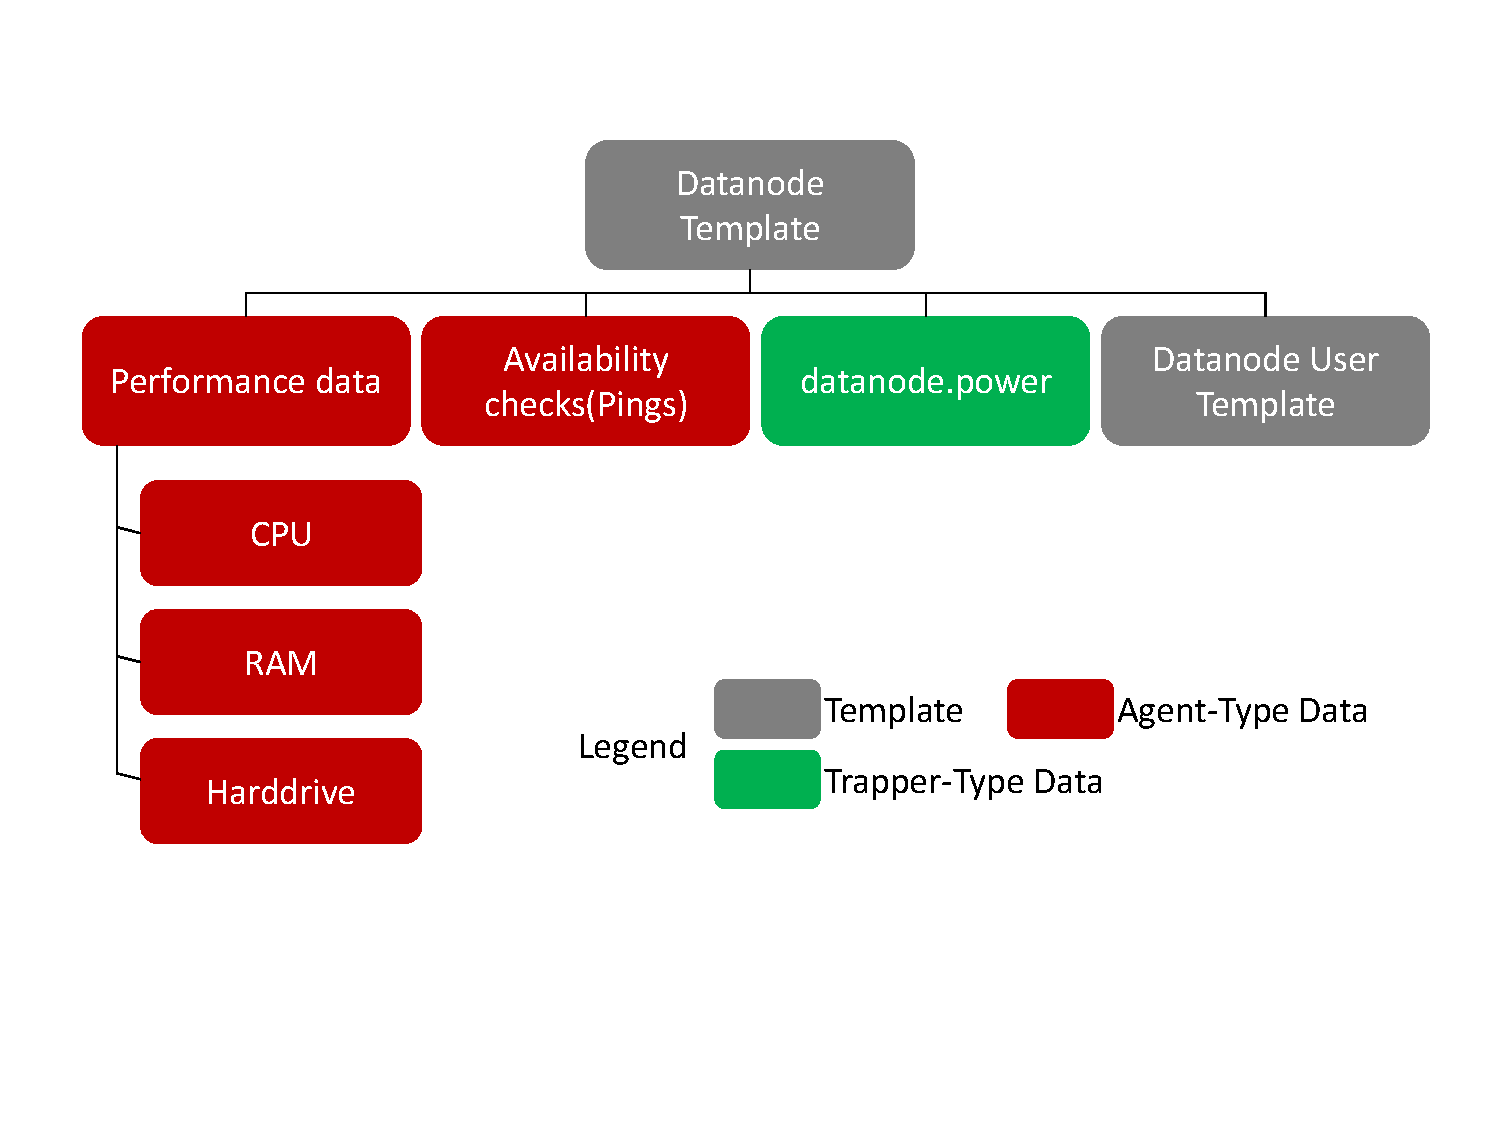
\includegraphics[width=0.5\textwidth]{img/ZabbixDatanodeTemp} 

\caption{Datatypes in the Zabbix Datanode Template}
\label{zabbix_datanode_template}
\end{figure}
	The server template was named "Cit Project Datanode" as to represent the datanode of the Hadoop distributed file systems data storage node. Within this template were items added from the Zabbix agent library to collect data on the monitored datanode shown in red in  figure \ref{zabbix_datanode_template}. These items were mostly Zabbix agent items to ease the collection of system load information data. The collected data were for example heartbeat pings to ensure the corresponding datanode can still be reached and did not disconnect or crash or CPU load distributions and allocated memory to monitor the overall load on the datanode for future analysis or optimized distributions of workloads among the utilized servers and many more load or simple check data types. For the purpose of collecting such data in an efficient manner it was chosen to use the Zabbix agent rather than trying to collect and send all these information by our own. The only manually collected and sent data field as a trapper type item was the "datanode.power" which represented the current voltage consumption for the corresponding datanode shown in green in figure \ref{zabbix_datanode_template}. This data was essential for the further analysis and calculations and as such was key data in the project.
\begin{figure}[ht]
\centering
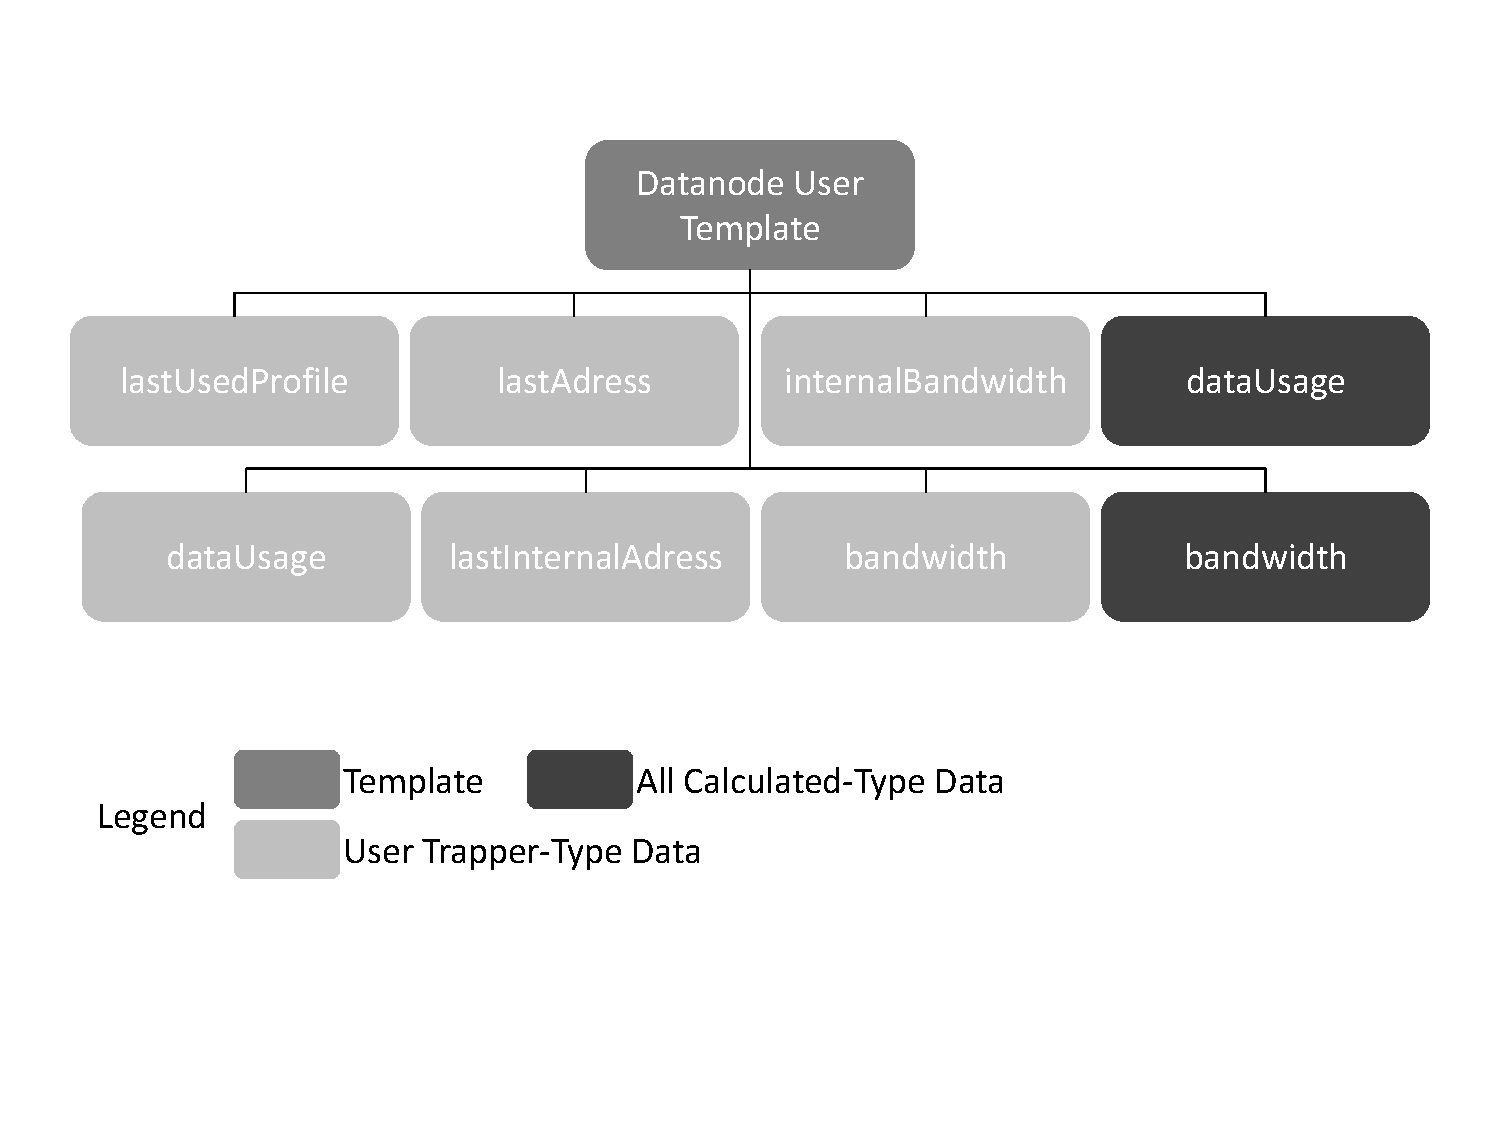
\includegraphics[width=0.5\textwidth]{img/ZabbixUserTemp} 

\caption{Datatypes in the Zabbix User Template}
\label{zabbix_user_template}
\end{figure}	
	The user template was named "Cit Project Datanode Users" as to represent all the necessary data items for user interaction on the system and assigned to the "Cit Project Datanode" template, shown as part of the Datanode Template in figure \ref{zabbix_datanode_template}, to allow the assignment of all necessary items to every datanode representation within Zabbix with a single template. Every user is represented through items shown in figure \ref{zabbix_user_template}, like "user.username.lastUsedProfile", "user.username.lastInternalAdress", "user.username.lastAdress", "user.username.internalBandwidth", "user.username.bandwidth" and "user.username.dataUsage". The item "user.username.lastUsedProfile" is necessary for the reporting to differentiate when the user used which kind of pricing profiles when he accessed the system. This way it is possible to calculate more precisely and fair how much expenses incurred from the users access. The items "user.username.lastInternalAdress" and "user.username.lastAdress" are for identifying the user communication stream in Software Defined Network flows to assign the resulting traffic to the right user. This is necessary since the user name information is only given once on the request to mount the distributed file system. The item "user.username.bandwidth" is representing the traffic from outside, like for example from his home, caused by the users' actions on the file system, like downloading or uploading of files. The item "user.username.internalBandwidth" however references to the traffic caused by the user which resulted from communication between the file systems data nodes for synchronization or replication of files the user had changed or created. Thus a sum of "user.username.bandwidth" and "user.username.internalBandwidth" would total the overall traffic caused by the user. Both items could be used to calculate the incurred costs from the users' activity on a single datanode. The last user item "user.username.dataUsage" is representing the allocated space on the file systems by the users' directories and files. This item is invaluable to determine the costs for the allocated space for when the user is not actively accessing the file system. All these user items are configured as trapper types to let Zabbix know that these items are being sent manually and it has to simply parse the information when it arrives. However there are two more user items, which are not specific to a single user, but rather to all users together. These are the two calculated items "user.all.dataUsage" and "user.all.bandwidth", shown in blue in figure \ref{zabbix_user_template}. These are as the names imply the summations of the last values of the items "user.username.dataUsage" and "user.username.bandwidth" as to give a comparative value for the total allocated space and caused traffic by all users and a  way to calculate the partial incurred traffic costs by a single user compared to the overall traffic.
	The Zabbix server however received his very own selection of templates from a wide range of predesigned templates within Zabbix. These templates had not only just regular server load specific data types, but also a great number of items to better monitor Zabbix functionality and load.
\begin{figure}[ht]
\centering
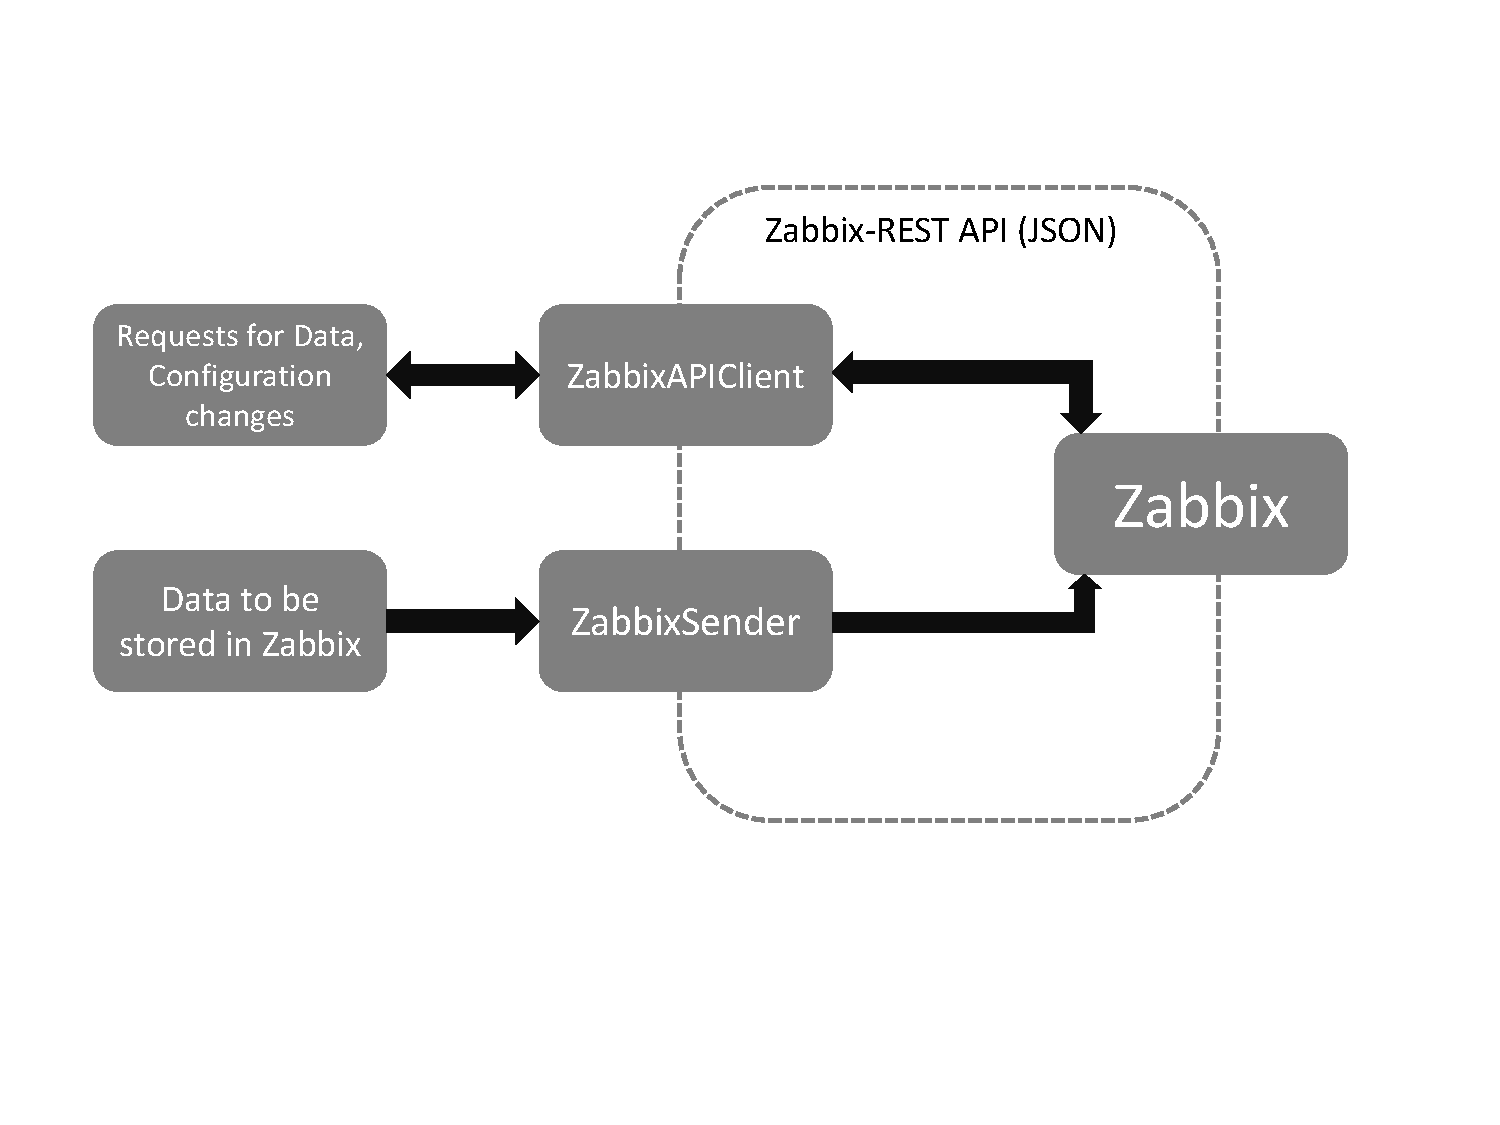
\includegraphics[width=0.5\textwidth]{img/ZabbixApiSender} 

\caption{Zabbix Communication Interface}
\label{zabbix_api_sender}
\end{figure}
	It was decided to create a unified interface for the communication with Zabbix. This was further split into two, the "ZabbixSender" and the "ZabbixAPIClient" as can be seen in figure \ref{zabbix_api_sender}. The "ZabbixSender" main task was to send trapper type data to Zabbix. The use of the command line prompt zabbix\_sender from Zabbix was canceled as the use from a JAVA program environment forked a new thread on every send just to execute the command line. This was deemed not efficient and further the zabbix\_sender required a library installation. It became obsolete as a method was found for packaging data into a JSON package and sending it directly to Zabbix from a JAVA program environment. Furthermore the "ZabbixSender" was set up as a static class which is working itself through a list of queued data transfers to Zabbix. The "ZabbixSender" is used as a one-way communication interface. The "ZabbixAPIClient" was created as a means of retrieving data from Zabbix for example for analysis or to change the configuration of Zabbix. Thus the "ZabbixAPIClient" housed among many the methods for data history retrieval, creating and deleting user items in the "Cit Project Datanode Users" template and the most important of them all the method for authenticating. "ZabbixAPIClient" was also set up as a static class to be continuously referenced and called but to be created only once. Both the "ZabbixSender" and the "ZabbixAPIClient" communicate with Zabbix using its REST API interface by sending remote procedure calls in the form of JSON packages back and forth.
The listing \ref{zabcode1} is an example of such a JSON package.
\begin{lstlisting}[language=json_sw,caption={JSON authentication request\cite{zab3}},captionpos=b,numbers=left,label=zabcode1]
{
    "jsonrpc": "2.0",
    "method": "user.login",
    "params": {
        "user": "Admin",
        "password": "zabbix"
    },
    "id": 1
}\end{lstlisting} 
	This is an example of the JSON remote procedure call of the method "user.login" sent to Zabbix. The field "id" is used to differentiate between calls to assign received results in the right way. The field "jsonrpc" simply gives the version of the JSON remote procedure calls. The field "params" holds all the information which is required for the method. In this case the only parameters are Zabbix login information. For other methods the parameters can be item ids, value or item names to be searched or filtered, whole definitions of new items or hosts for item or host creation, updated formulas for calculations or graph items for graphs, flags or database expressions and many more. The JSON request after being constructed is then put into the body of an http client post with a modified header so that the request would be received correctly and then sent to Zabbix. If Zabbix receives the JSON package and the formatting was correct, the method existed and the parameters were fitting the method, then Zabbix would return the result packaged in another JSON package like the example in listing \ref{zabcode2} for the JSON remote procedure call from listing \ref{zabcode1}.
	\begin{lstlisting}[language=json_sw,caption={JSON authentication response\cite{zab3}},captionpos=b,numbers=left,label=zabcode2]
{
    "jsonrpc": "2.0",
    "result": "0424bd59b807674191e7d77572075f33",
    "id": 1
}
\end{lstlisting}
	As can be seen, this result yielded just a long authentication token, which in turn is necessary as another field next to "jsonrpc", "params" or "method" for many other methods, since they are requiring a certain level of rights \cite{zab3}. Thus this authenticate token can be used instead of sending the login data every single time and thus creating a risk of them being compromised.
	A great number of configuration definitions, like item names, template names, Zabbix login information, Zabbix URL and ports, are stored for flexibility and ease of modifications in the "ZabbixParams" class. This class stores the configuration information of Zabbix to keep the "ZabbixSender" and the "ZabbixAPIClient" free of hard-coded names.
\subsubsection{Conclusion}
	Zabbix as a monitor did fulfill the requirements and it was possible to realize some of the goals, like full data model representation, creation of communication interfaces with Zabbix, visualization of great number of data types, functioning triggers, a plethora of server load specific data types, successful identification of user traffic using the IP address. However there were spots where Zabbix did not shine as much as it would have been desired. For instance, calculated items creation in the web front end only works if the formula is not empty, however through the REST API it is possible to empty it altogether, making one wonder why the web front end forbids doing so. Furthermore calculated items are prone to becoming unsupported thus being disabled for a certain span of time if some of the fields in the formula of the calculated item have no values. In general the REST API, despite its usefulness, has the tendency to result in hard to overview program code, not mentioning the quite picky habits of Zabbix to which parameters it wants to succeed the remote procedure call execution. Another though albeit really small issue is with the visualization of trapper data in graphs. If the graph received some data after a longer time span it simply connects the previous value with the new one even if the data in between could have been zero but it was not deemed necessary to send a few zeros.
	All in all Zabbix did its job although with some ups and downs. It is truly hard to say whether Zabbix was or was not a well suited choice without having it undergo a test in a more or less realistic environment with dozen or even hundred of servers with a great number of users to see if Zabbix actually can run stable without being overloaded. Only such a long term observation could yield insight into the trending of data or possible energy conservation, perhaps even the knowledge on how to reiterate the data model or proof for reconsideration of the choice on Zabbix. Such information is hard to discover about the project as a whole in its current state, as the testing environment was quite small and for an endeavor of such big scale insufficient.